% OCR draft from PDF pages 220-234 (book chapter 7).
\chapter{A Simulation Environment}
\label{chap:simulation-environment}

\section{Introduction}
\label{sec:simenv-intro}

This chapter presents a user-level view of the SMPL simulation environment.
SMPL includes:
\begin{itemize}
\item the \texttt{smpl} subsystem from Chapter 2,
\item debugging/analysis/reporting tools,
\item an interactive run-time interface called \texttt{mtr}.
\end{itemize}

In the implementation described (SMPL/PC), \texttt{mtr} acts as the interactive
front-end between user, simulation model, and support modules.

\begin{figure}[ht]
\centering
\begin{tikzpicture}[>=Latex,node distance=1.3cm and 1.6cm]
  \node[draw,minimum width=2.8cm,minimum height=1cm] (user) {User};
  \node[draw,minimum width=3.4cm,minimum height=1cm,right=of user] (mtr) {\texttt{mtr} interface};
  \node[draw,minimum width=3.3cm,minimum height=1cm,right=of mtr] (model) {Simulation model};
  \node[draw,minimum width=3.0cm,minimum height=1cm,below=of model] (smpl) {\texttt{smpl} core};
  \node[draw,minimum width=2.3cm,minimum height=0.9cm,below=of user] (dump) {\texttt{dump}};
  \node[draw,minimum width=2.3cm,minimum height=0.9cm,right=0.8cm of dump] (table) {\texttt{table}};
  \node[draw,minimum width=2.3cm,minimum height=0.9cm,right=0.8cm of table] (bma) {\texttt{bma}};
  \node[draw,minimum width=2.3cm,minimum height=0.9cm,right=0.8cm of bma] (dis) {\texttt{dis}};
  \node[draw,minimum width=2.3cm,minimum height=0.9cm,below=0.9cm of table] (parms) {\texttt{parms}};

  \draw[<->,line width=0.95pt] (user) -- (mtr);
  \draw[<->,line width=0.95pt] (mtr) -- (model);
  \draw[<->,line width=0.95pt] (model) -- (smpl);
  \draw[<->,line width=0.9pt] (mtr.south) -- (dump.north);
  \draw[<->,line width=0.9pt] (mtr.south) -- (table.north);
  \draw[<->,line width=0.9pt] (mtr.south) -- (bma.north);
  \draw[<->,line width=0.9pt] (mtr.south) -- (dis.north);
  \draw[<->,line width=0.9pt] (mtr.south) -- (parms.north);
  \draw[<->,line width=0.9pt] (smpl.west) -- ++(-0.9,0) |- (dump.east);
  \draw[<->,line width=0.9pt] (smpl.west) -- ++(-0.4,0) |- (table.east);
  \draw[<->,line width=0.9pt] (smpl.east) -- ++(0.4,0) |- (bma.west);
  \draw[<->,line width=0.9pt] (smpl.east) -- ++(0.9,0) |- (dis.west);
\end{tikzpicture}
\caption{The SMPL Simulation Environment}
\label{fig:smpl-environment}
\end{figure}

Main optional modules:
\begin{itemize}
\item \textbf{dump}: event list, queue contents, facility users/status.
\item \textbf{table}: table definition, entry, reports, and plots.
\item \textbf{bma}: batch means analysis for run-length control.
\item \textbf{parms}: named parameter definition and access.
\item \textbf{dis}: graphics display (time series and parameter plots).
\end{itemize}

\section{The Run-Time Interface}
\label{sec:simenv-mtr}

The simulation program chooses whether \texttt{mtr} is active (via
\texttt{smpl()} options), so production runs can bypass interaction.

When enabled, \texttt{mtr} pauses:
\begin{enumerate}
\item after initial \texttt{smpl} initialization (for parameter/table setup),
\item after first event scheduling (when facilities exist; useful for display
  setup).
\end{enumerate}

During execution, \texttt{mtr} can pause on user input, display completion,
model breakpoints, or errors. While running, it monitors each event boundary:
breakpoint checks, active analysis/display updates, and function-key polling.

\begin{figure}[ht]
\centering
\begin{tabular}{lll}
\toprule
Key & Action & Typical use \\
\midrule
F1 & Pause/continue & Enter interactive mode at runtime \\
F2 & Toggle trace & Event-by-event debugging \\
F3 & \texttt{dump} display & Inspect facilities/queues/events \\
F4 & Report display & View cumulative performance measures \\
F5 & Table setup & Configure distribution sampling \\
F6 & BMA setup & Configure sequential run-length control \\
F7 & Graphics setup & Configure \texttt{dis} plotting mode \\
F8 & Parameter edit & Change model parameters during run \\
F9 & Breakpoint control & Stop on condition/time/event \\
F10 & User display hook & Invoke model-defined display routine \\
\bottomrule
\end{tabular}
\caption{SMPL/PC Function Keys}
\label{fig:smpl-function-keys}
\end{figure}

Representative controls include pause/continue, trace toggles, dump/report
display, table/bma/dis setup, parameter display/edit, breakpoint control, stream
selection, and optional user-defined display function invocation.

\section{Parameters}
\label{sec:simenv-parameters}

SMPL parameters are named real-valued variables registered by the model and
shared with \texttt{mtr} and modules via the \texttt{parms} registry.

Benefits:
\begin{itemize}
\item reduces custom input/report coding in models,
\item allows keyboard display/modification of selected model variables,
\item provides direct inputs for table/bma/dis,
\item supports parameter-based breakpoints.
\end{itemize}

\section{The \texttt{dump} Module}
\label{sec:simenv-dump}

\texttt{dump} displays the current simulator state:
\begin{itemize}
\item per-facility server state and reserving token/priority,
\item queue contents (event/token/priority/time-left),
\item queue activity timestamps,
\item event list entries and last-caused event.
\end{itemize}

It can be invoked by model call, function key, or automatically on simulator
error.

\begin{figure}[ht]
\centering
\fbox{%
\begin{minipage}{0.9\textwidth}
\small\verbatimfont
time = 15200.00 \quad last event = 2 \quad token = 17\\
------------------------------------------------------------\\
FACILITY STATUS\\
cpu\#1 : busy by token 17 \quad qlen=3 \quad util=0.87\\
cpu\#2 : idle \quad qlen=0 \quad util=0.55\\
disk\#1: busy by token 09 \quad qlen=1 \quad util=0.71\\
disk\#2: busy by token 21 \quad qlen=2 \quad util=0.68\\
------------------------------------------------------------\\
EVENT LIST (next 6)\\
(t=15201.32,e=2,tk=17)\quad (t=15202.04,e=1,tk=41)\\
(t=15202.67,e=4,tk=09)\quad (t=15203.90,e=2,tk=21)\\
\end{minipage}}
\caption{\texttt{dump} Module Output Example}
\label{fig:smpl-dump-example}
\end{figure}

\section{The \texttt{table} Module}
\label{sec:simenv-table}

\texttt{table} provides histogram-like collection/reporting:
\begin{itemize}
\item define value range and interval count,
\item enter observations,
\item report mean/stddev and interval frequencies/cumulative frequencies,
\item optionally plot the table.
\end{itemize}

Tables can be model-defined (entries by function call) or \texttt{mtr}-defined
(entries by parameter/count observation). A single \texttt{mtr}-driven table is
supported to keep monitoring overhead low.

\section{The Batch Means Analysis Module}
\label{sec:simenv-bma}

\texttt{bma} estimates run length for a target relative confidence-interval
half-width on a discrete-time output variable.

Workflow:
\begin{enumerate}
\item discard initial observations (\emph{warm-up}),
\item collect initial batches and test lag autocorrelation,
\item if dependent, merge adjacent batches (doubling batch size),
\item when independence is acceptable, keep adding batches until target
  relative half-width is met,
\item optionally reduce final batch count (to improve coverage) while
  preserving target accuracy.
\end{enumerate}

Input setup (from \texttt{mtr} or model code) includes output/count parameters,
warm-up count, initial batch size/count, target relative half-width, confidence
level, lag-count, significance level, and max-observation limit.

\begin{figure}[ht]
\centering
\begin{minipage}{0.47\textwidth}
  \centering
  \fbox{%
  \begin{minipage}{0.9\textwidth}
  \small\verbatimfont
  BMA INPUT\\
  output parameter: \texttt{queue\_len}\\
  count parameter : \texttt{n\_obs}\\
  warm-up count   : 1000\\
  initial batch   : 200\\
  initial batches : 16\\
  confidence      : 0.95\\
  target rel H/W  : 0.10\\
  lag test count  : 8\\
  alpha test      : 0.05
  \end{minipage}}
\end{minipage}\hfill
\begin{minipage}{0.47\textwidth}
  \centering
  \fbox{%
  \begin{minipage}{0.9\textwidth}
  \small\verbatimfont
  BMA OUTPUT\\
  merged batch size: 800\\
  independent lags : pass\\
  batches used     : 28\\
  mean             : 4.217\\
  std error        : 0.108\\
  CI half-width    : 0.226\\
  relative H/W     : 0.054\\
  run status       : target met
  \end{minipage}}
\end{minipage}
\caption{\texttt{bma} Input and Output Displays}
\label{fig:smpl-bma}
\end{figure}

The chapter notes that batch-means methods are empirical tools and should be
used with care; it references broader output-analysis comparisons.

\section{The Graphics Display Module}
\label{sec:simenv-dis}

\texttt{dis} provides interactive plots, including:
\begin{itemize}
\item facility utilization vs.\ time,
\item average queue length vs.\ time,
\item current queue length vs.\ time,
\item parameter vs.\ time,
\item parameter vs.\ parameter/count.
\end{itemize}

Plots are configured from an input panel (option-specific parameters such as
facility/parameter IDs, axis ranges, time span, plotting mode). Data can also be
written to file for external plotting.

\begin{figure}[ht]
\centering
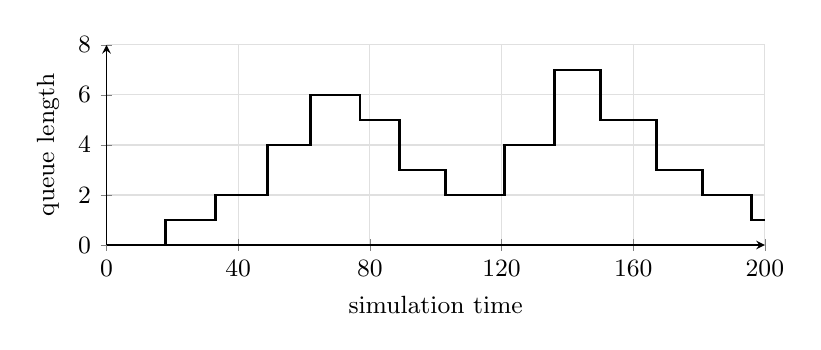
\begin{tikzpicture}
\begin{axis}[
  width=0.82\textwidth,height=0.34\textwidth,
  xmin=0,xmax=200,ymin=0,ymax=8,
  axis lines=left,
  xlabel={simulation time},
  ylabel={queue length},
  xtick={0,40,80,120,160,200},
  ytick={0,2,4,6,8},
  ticklabel style={font=\small},
  label style={font=\small},
  grid=major,
  major grid style={draw=black!12}
]
\addplot[const plot,line width=1pt] coordinates {
  (0,0) (18,1) (33,2) (49,4) (62,6) (77,5) (89,3) (103,2)
  (121,4) (136,7) (150,5) (167,3) (181,2) (196,1) (200,1)
};
\end{axis}
\end{tikzpicture}
\caption{\texttt{dis} ``step mode'' Plot}
\label{fig:smpl-dis-step}
\end{figure}

Typical uses: warm-up estimation, ad hoc run-length checks, dynamic behavior
inspection, and bug discovery via live trend observation.

\section{Summary}
\label{sec:simenv-summary}

The chapter's core point is productivity: parameterization plus interactive
control reduce code/compile/debug cycles and support rapid model experimentation.
With \texttt{mtr}, \texttt{parms}, and optional analysis/display modules, many
studies can be run with little or no model recoding. The implementation details
are system-dependent mostly in UI/display glue, making portability practical.
